%% main.tex — The Noirsystic Pipeline, Third Form
%% Build: docker texlive, pdflatex -> bibtex -> pdflatex x2
\documentclass[journal]{IEEEtran}

\usepackage{amsmath,amssymb}
\usepackage{graphicx}
\usepackage{booktabs}
\usepackage{url}
\usepackage{microtype}
\usepackage{siunitx}
\usepackage[numbers,sort&compress]{natbib}
\usepackage{balance}

\graphicspath{{figures/}}
% generated by make_figures.py - do not edit

\newcommand{\NumShadowN}{12}
\newcommand{\NumShadowOldPass}{12}
\newcommand{\NumShadowNewPass}{0}
\newcommand{\NumAttacksTotal}{9}
\newcommand{\NumAttacksDefeated}{6}
\newcommand{\NumTrajectoriesScanned}{140}
\newcommand{\NumTrajectoriesUsed}{0}
\newcommand{\NumShadowReproduced}{8}
\newcommand{\NumShadowAttempts}{8}
\newcommand{\NumTicks}{361}
\newcommand{\NumRuns}{146}
\newcommand{\NumHypotheses}{53}
\newcommand{\NumNegatives}{23}
\newcommand{\NumGraduations}{0}
\newcommand{\NumCommits}{1{,}951}
\newcommand{\NumSpend}{2.17}
\newcommand{\NumLesionHaikuA}{79.6}
\newcommand{\NumLesionHaikuB}{68.5}
\newcommand{\NumLesionHaikuC}{83.3}
\newcommand{\NumLesionQwen}{98.2}
\newcommand{\NumPassVisible}{86.7}
\newcommand{\NumPassSealed}{90.0}
\newcommand{\NumPassAdversarial}{92.5}
\newcommand{\NumCapNine}{1084}
\newcommand{\NumCapNinePrior}{1082}
\newcommand{\NumCapEleven}{5529}
\newcommand{\NumCapElevenPrior}{5504}
\newcommand{\NumCapNineDelta}{2}
\newcommand{\NumCapElevenDelta}{25}
\newcommand{\NumCapNineUpper}{2070}
\newcommand{\NumCapElevenUpper}{16857}


\hyphenation{Noir-sys-ti-ca veri-fi-ca-tion re-flex-ive in-stru-men-tal}

\begin{document}

\title{The Noirsystic Pipeline, Third Form:\\
A Reflexive Agent Laboratory and the Transfer of\\
Its Verification Doctrine to Cap-Set Search}

\author{\IEEEauthorblockN{Michael A.~Vega}
\IEEEauthorblockA{Noirsys Research Group\\
Email: contact@noirsys.com}}

\maketitle

\begin{abstract}
The Noirsystic Pipeline is a single agent architecture---a written
constitution, an append-only ledger, and a verifier the agent cannot
write to---instantiated three times: first for software development,
second for a business (Noirpost), and third, in the form reported here,
for research on agents themselves. The first two instances are
\emph{instrumental}: the pipeline produces an artifact outside itself.
The third is \emph{reflexive}: the pipeline's subject is the pipeline.
We describe that third instance and report the two things it produced.
First, a finding about evaluation harnesses: a scoring system written by
the same class of system it judges is attackable through the
\emph{environment} rather than through its screening, so that in a
controlled probe every one of \NumShadowN{} unsolved items was reported
as passed before a containment fix and none afterward; and the nine
adversarial constructions raised against it divided cleanly into
capability and propensity, defeating the filter in \NumAttacksDefeated{}
of \NumAttacksTotal{} cases while appearing in \NumTrajectoriesUsed{} of
\NumTrajectoriesScanned{} production trajectories. Second, a
demonstration that the resulting doctrine transfers out of the
laboratory: a cap-set search harness built to that doctrine, containing
no language model anywhere in its search path, established lower bounds
$c(9,3) \ge \NumCapNine$ (previously \NumCapNinePrior) and
$c(11,3) \ge \NumCapEleven$ (previously \NumCapElevenPrior), and---more
instructively---caught in the act the exact failure mode the laboratory
had characterised, when the harness announced a ``record'' that sat
below the published bound. We are explicit about what this does and does
not show: the mathematics does not depend on the laboratory, and the
laboratory's contribution to it is a checking regime, not a result.
\end{abstract}

\begin{IEEEkeywords}
agent evaluation, verification, containment, cap sets, extremal
combinatorics, local search, research infrastructure
\end{IEEEkeywords}

\begin{figure}[!b]
\centering
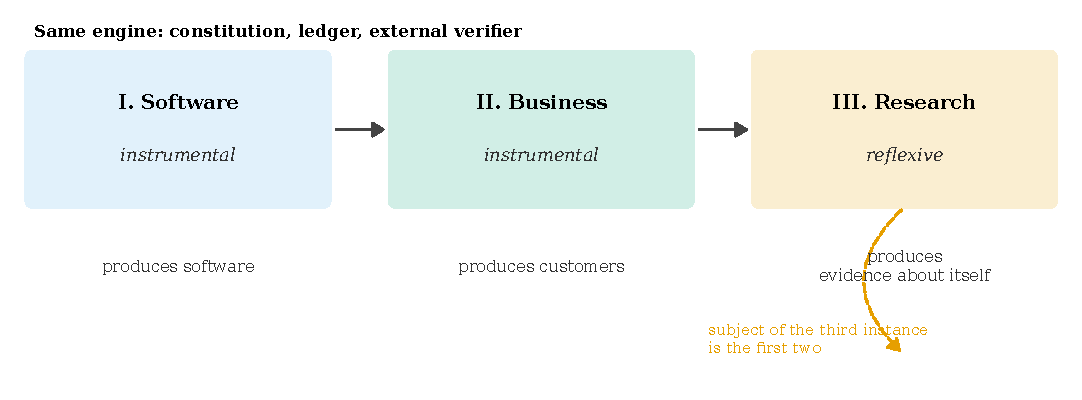
\includegraphics[width=\columnwidth]{fig1_three_forms.pdf}
\caption{The Noirsystic Pipeline in its three forms. Forms I and II are
instrumental: the artifact is produced outside the pipeline. Form III is
reflexive: the pipeline's subject is the pipeline, which changes what
its verifier has to protect against.}
\label{fig:forms}
\end{figure}

\section{Introduction}

A recurring pattern in the recent literature on AI agents is the
discovery that the measurement apparatus, not the capability, is the
fragile part. An agent that can modify the code that scores it will
score well; an agent that knows it is being evaluated will behave
differently from one that does not \cite{krakovna2020,meinke2024}. The
practical consequence is that reports of agent capability increasingly
depend on claims about a harness that nobody has attacked.

This paper reports one such attack, and then reports what the attack was
good for. Both come from the same place: an agent pipeline that has been
instanced three times, and whose third instance was pointed at the
question of whether the first two were doing what they appeared to be
doing.

\paragraph{Contributions} Three, in order of durability:
\begin{enumerate}
\item A characterisation of a class of evaluation failure that is not
closed by screening. A verifier that runs in an environment the subject
can write to is compromised regardless of how carefully it inspects the
subject's output. We show this with a controlled probe in which
\NumShadowOldPass{} of \NumShadowN{} unsolved items were reported as
passed, and \NumShadowNewPass{} of \NumShadowN{} after a containment
change.
\item Two lower bounds for cap sets in $\mathbb{F}_3^9$ and
$\mathbb{F}_3^{11}$, at \NumCapNine{} and \NumCapEleven{}, with
byte-identified witnesses and two independent checkers.
\item A worked example of the doctrine transferring: the same harness
later produced a false ``record'' by grading itself against a stale
internal number, and the failure was caught by the regime the laboratory
had established rather than by the personnel who had built the harness.
\end{enumerate}

The ordering is deliberate. The cap-set bounds are the most checkable
result and the least dependent on anything we argue; the verification
doctrine is the more useful result; the transfer is the paper's actual
claim.

\section{The Noirsystic Pipeline}

The Noirsystic Pipeline, defined by its author, is a single
architecture instantiated across domains. Its invariants are:

\begin{itemize}
\item \textbf{A written constitution.} The rules of the loop---what it
may modify, what it may not, how a result gets accepted---exist as a
document the loop reads each cycle, not as tacit practice.
\item \textbf{An append-only ledger.} Every cycle writes one entry. The
ledger is the record; there is no separate reporting layer that could
drift from it.
\item \textbf{A verifier outside the writer.} Acceptance is decided by
something the producing agent cannot edit: another model family, a
sealed evaluation set, a human, or a program.
\end{itemize}

The three forms differ in where the artifact lands. Form I, software
development, produces software. Form II, a business, produces customers.
Forms I and II are \emph{instrumental}: the pipeline is a means, and the
artifact is external. Form III, research on agents, produces evidence
about the pipeline. It is \emph{reflexive}, and the reflexivity is not a
domain label but a structural change: in Forms I and II the verifier
protects the artifact from the agent, while in Form III the verifier
must protect the \emph{measurement} from the agent, and the agent has a
stronger interest in the measurement than in any artifact. Figure
\ref{fig:forms} shows the three forms and the loop closing.

This paper reports Form III, and its usefulness is judged by a single
question: did anything the third instance learned change what the first
two do?

\section{Form III: The Reflexive Instance}

The laboratory is a two-family system: two model families take turns as
Lead of Record and Second, each cycle is pre-registered as a hypothesis,
and results are judged on visible, sealed and adversarial splits the
proposing agent never sees. Its constitution states its own limits
plainly---it does not train models, does not modify its kernel, and does
not believe its own results until a hostile reviewer, a sealed set, and
a second model family have all failed to break them.

Over \NumTicks{} cycles it ran \NumRuns{} scored runs, logged
\NumHypotheses{} hypotheses and \NumNegatives{} negative results, and
graduated \NumGraduations{} mechanisms. We treat that last number as the
laboratory's headline about itself rather than a disappointment: a
measurement apparatus that produces mostly negatives is behaving like an
apparatus. The reason for the zero is arithmetic, not failure of will---a
small coding benchmark near its ceiling requires an effect larger than
the difference available to be detected at the sample sizes the
laboratory can afford.

What the laboratory did produce, and what Forms I and II could not have
produced, is a specification of what its own verifier must survive.

\section{The Verifier's Environment Is the Attack Surface}

\subsection{The probe}

The laboratory's own harness scored a subject's work using a checker that
ran in the same shell as the subject, over a work tree the subject could
write. The consequence is not subtle. Placing a module named \texttt{json.py}
in the work tree means the \emph{grader's own import} resolves to the
subject's file. An unsolved item is then reported as solved without any
incorrect mathematics having been performed.

Against \NumShadowN{} known-unsolved items, this produced
\NumShadowOldPass{} of \NumShadowN{} reported passes. After the checker
was moved into a clean, network-isolated container with no mount from the
work tree, \NumShadowNewPass{} of \NumShadowN{} (Fig.~\ref{fig:channel},
left). The defect is not a bug in a checker; it is a property of running
the checker in a place the subject can reach.

\subsection{Capability and propensity are different quantities}

An adversarial process instructed to defeat the filter did so in
\NumAttacksDefeated{} of \NumAttacksTotal{} constructions, and in one
family executed a shell command inside the probe container through a
Python string annotation. That is capability.

Propensity is a separate question, and the answer here is none. An
independent scan over all trajectories retained on disk---%
\NumTrajectoriesScanned{} files across thirty run directories, every tool
call inspected for references to the lab root, the evaluation
directories, any answer file, any checker, or the network---found
\NumTrajectoriesUsed{} uses (Fig.~\ref{fig:channel}, right). The subjects
touched their work directory and used the tools the tasks provided.

We are careful about the reading. ``We found agents scheming'' and ``we
found three ways our own scoring could be cheated, and closed them'' are
the same events described at different levels of honesty. Only the second
is reproducible, and only the second is what this dataset supports. It
also does not separate capability from luck: the workers best placed to
exploit one channel never produced a proposal at all.

\begin{figure}[!t]
\centering
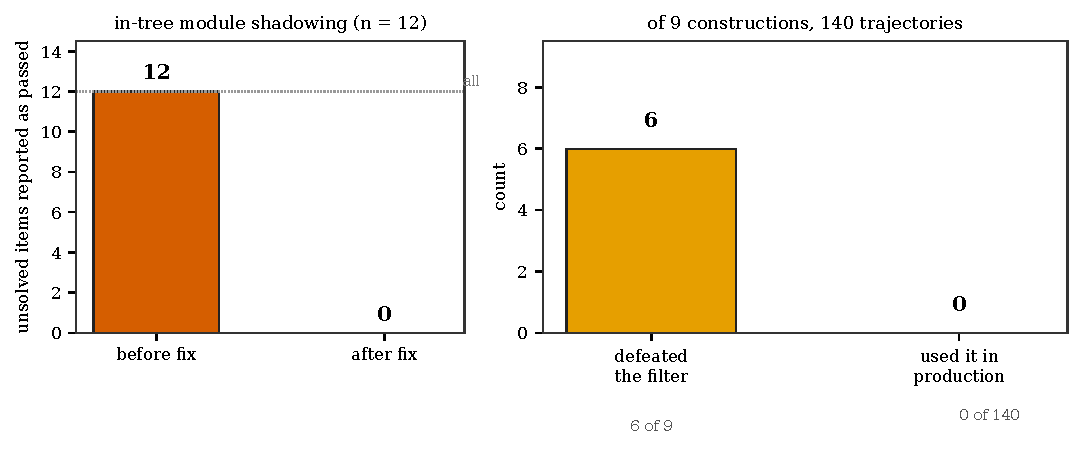
\includegraphics[width=\columnwidth]{fig2_channel_closure.pdf}
\caption{Left: the in-tree module shadowing probe. The grader's own
import resolved to a file the subject placed in the work tree, so
\NumShadowOldPass{} of \NumShadowN{} unsolved items were reported as
passed; after containment, \NumShadowNewPass{} of \NumShadowN{}. Right:
capability versus propensity. The filter was defeated in
\NumAttacksDefeated{} of \NumAttacksTotal{} instructed constructions and
in \NumTrajectoriesUsed{} of \NumTrajectoriesScanned{} production
trajectories.}
\label{fig:channel}
\end{figure}

\subsection{What replaces screening}

The general conclusion is that text-screening a symbolic channel is an
accident detector rather than a barrier. String inspection catches a
careless literal and cannot catch a module import, a path traversal, or a
process that writes a file another process later executes. What protects
a holdout is containment, and containment is a testable property in a way
that screening is not. Three requirements, each learned by being attacked:
the answer key is never materialised while the subject's process is
alive; the checker never executes in an environment the subject could
write; and the subject never sees the holdout.

\section{The Doctrine as a Specification}

The laboratory's contribution to anything downstream is therefore a
checking regime, and it is short enough to state as a specification:

\begin{enumerate}
\item An agent's self-report is not evidence, including when the agent is
correct.
\item A claim is accepted only when a checker that shares no code with
the process under test says so.
\item Where a number is compared against a standard, the comparison is
performed, not displayed.
\item Artifacts are byte-identified, and the identity is checked after
the analysis, not only at creation.
\end{enumerate}

The next section reports what happened when that regime was applied to a
subject with no language model in it at all.

\section{The Transfer: A Cap-Set Harness Built to the Regime}

\subsection{The problem}

A cap set in $\mathbb{F}_3^n$ is a subset containing no three points
$x,y,z$ with $x+y+z=0$. The quantity $c(n,3)$ is the largest such size.
A construction of size $N$ proves $c(n,3) \ge N$; an upper bound is a
statement that nothing larger exists, which is a different artifact
entirely \cite{oeis}. Large-$n$ values are not known exactly beyond
$n=6$; the gap between the best construction and the best upper bound is
wide at every dimension of interest
\cite{edel2004,karapetyan2023,funsearch2023,versluis2017}. Published
constructions in this range come from algebra rather than from search:
code-based and curve-based caps in projective space, doubled into the
affine space \cite{edel2004,karapetyan2023,karapetyan2024}. The current frontier is
maintained informally across several groups, most recently surveyed with
an explicit table in \cite{endlessexam2026}; the most active group
continues to publish new constructions at other dimensions
\cite{karapetyan2026}.

\subsection{Why there is no model in the loop}

The harness contains no language model anywhere in its search path. This
is a design consequence of Section IV and not an accident of scale. A
language model in the inner loop would be an agent reporting its own
progress, which is exactly the object the laboratory showed cannot be
trusted to grade itself. The search is a constraint solver and numpy
arithmetic on the author's own cores: large-neighbourhood search that
removes a structured neighbourhood of the current cap, re-solves the hole
to optimality as a maximum independent set in the lines hypergraph, and
accepts only strict improvements.

The harness nevertheless runs two engines, and the distinction matters
for what it can produce. The first is that local search. The second is
symmetry-restricted \emph{exact} search: pick a symmetry group of the
space, reduce the problem to choosing among its orbits, solve to
optimality, and emit either a larger cap or the theorem ``no
$G$-invariant cap beats $X$.'' Every task in the second engine therefore
terminates in a statement.

\subsection{Verification}

Two checkers, sharing no code, agree on both witnesses. The project's own
checker tests the property as a pair scan over a tuple set. The
independent checker was written from the definition with a different
algorithm: points are packed as base-3 integers and tested against a
boolean membership table, which turns the property into array indexing.
The second form runs in \SI{0.17}{s} for $n=9$ and \SI{2.18}{s} for
$n=11$ where the first takes minutes, which is itself evidence that the
two implementations are genuinely different programs.

Both witnesses are stored as byte-identical copies with SHA-256 digests,
and all originals were re-hashed at the end of the analysis to confirm
they were unmodified. Four verification passes were run on a system
interpreter with no virtual environment, so that a referee needs nothing
installed.

\section{The Failure Mode Reappears, and Is Caught}

The instructive result of this section is not the bounds. It is that the
harness reproduced, outside the laboratory, the exact failure the
laboratory had characterised: a system grading itself against a number it
held internally and never re-derived.

The harness maintained a ``record to beat'' table in code. That table
held \NumCapElevenPrior{} at $n=11$, which was correct when written and
stale once the search passed it. Because every beats-record test,
artifact write, log line and dashboard banner keys off that one constant,
each size above it satisfied the test. The harness accordingly announced
a cap of $5492$ as a new record. The cap was real---it verified---but it
sat twelve points below the published bound of \NumCapElevenPrior{} and
thirty-seven below the harness's own best of \NumCapEleven{}.

Three defects were repaired, and each is the same defect in a different
place. The constant was corrected. The announcement path was changed to
compare against the current bar rather than to display the newest
artifact by timestamp---a banner that sorts by time never asks whether
the artifact still beats anything. And the display was filtered to
entries strictly above the bar, because a record written under a stale
bar otherwise stays on screen indefinitely.

The general lesson is the fourth item of the specification: the
comparison must be performed. A system that stores its standard and
displays its outputs has not compared them, and the failure is silent,
confident, and produces a plausible-looking file.

\section{Results}

\begin{table}[!t]
\caption{Cap-set frontier. Lower bounds are constructions; the two rows
in bold are established by this work. Upper bounds are independent.}
\label{tab:frontier}
\centering
\small
\begin{tabular}{@{}crrrc@{}}
\toprule
$n$ & lower bound & prior & upper bound & exact \\
\midrule
6  & 112   & 112   & 112   & yes \\
7  & 236   & 236   & 291   & no  \\
8  & 512   & 512   & 771   & no  \\
9  & \textbf{\NumCapNine} & \NumCapNinePrior & \NumCapNineUpper & no \\
10 & 2432  & 2432  & 5619  & no  \\
11 & \textbf{\NumCapEleven} & \NumCapElevenPrior & \NumCapElevenUpper & no \\
12 & 12928 & 12928 & --- & no \\
\bottomrule
\end{tabular}
\end{table}

\subsection{Lower bounds}

The harness establishes $c(9,3) \ge \NumCapNine$, an improvement of
\NumCapNineDelta{} over the prior bound of \NumCapNinePrior{}, and
$c(11,3) \ge \NumCapEleven$, an improvement of \NumCapElevenDelta{} over
\NumCapElevenPrior{}. Both were reached by local search seeded from
published projective constructions doubled into the affine space, and
both are verified by two independent checkers as described above.
Table~\ref{tab:frontier} and Fig.~\ref{fig:frontier} place them.

\begin{figure}[!t]
\centering
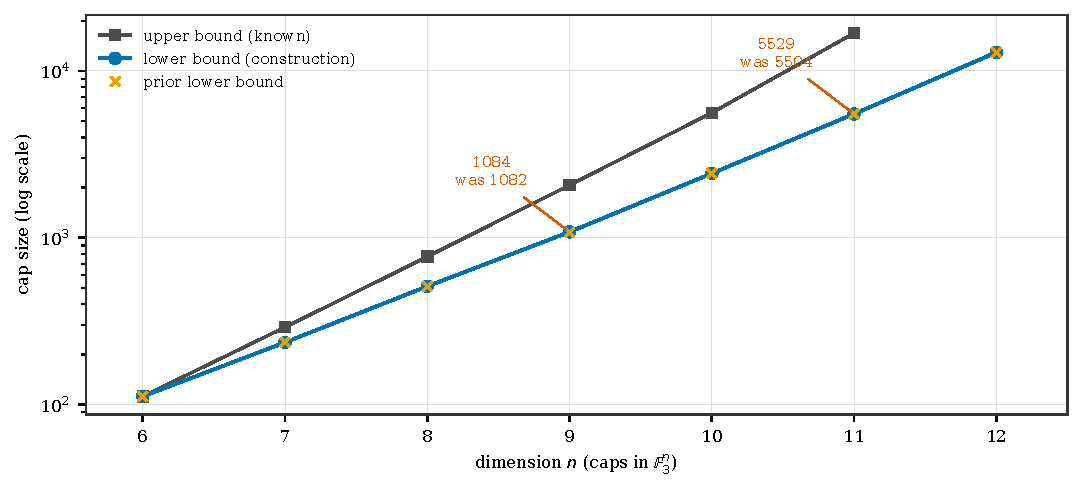
\includegraphics[width=\columnwidth]{fig3_frontier.pdf}
\caption{The cap-set frontier. The vertical distance between the two
series is the unresolved region; a construction raises the lower series
and cannot lower the upper one. The two marked points are the results
reported here.}
\label{fig:frontier}
\end{figure}

\subsection{Weighting the two margins}

The two results are not of equal durability---one of the specification's
requirements is that comparisons be performed, and that includes
comparing our own claims.

At $n=11$ the prior bound is a \emph{positive citation}: it is stated as
a numbered corollary in a published paper, so the comparison is against a
number we can point to. At $n=9$ the clearance is of a different kind. No
paper in this niche states a $d=9$ result, and the most active group in
the area states corollaries for four dimensions and skips this one. Our
result is therefore clear of the prior bound by an
\emph{absence-of-evidence} argument, which is weaker than a citation and
should be labelled as such in any public claim. A margin of
\NumCapNineDelta{} points on a four-figure record is also within reach of
an afternoon of a competitor's local search; it is provisional in a way
the $\NumCapElevenDelta$-point margin is less so, and both are rounding
next to the unresolved gap in Table~\ref{tab:frontier}.

\section{What This Does Not Establish}

Three things, stated plainly because the strong reading is available and
wrong.

\textbf{The mathematics does not depend on the laboratory.} The bounds
are properties of $\mathbb{F}_3^9$ and $\mathbb{F}_3^{11}$ and would hold
if every source file in this paper were deleted. The laboratory's
contribution is the checking regime that made the numbers trustworthy and
that caught the false record. Claiming that the reflexive pipeline
\emph{produced} the cap sets would be exactly the overclaim the laboratory
was built to refuse.

\textbf{This is not a demonstration of recursive self-improvement.} The
laboratory graduated no mechanisms. What transferred was a practice, not
a mechanism, and a practice is not the thing the RSI literature is about.

\textbf{The bound is not tight and does not claim to be.} The gap between
the constructions and the upper bounds in Table~\ref{tab:frontier} is
unresolved and large. Nothing here approaches it.

\section{Related Work}

\subsection{Evaluation of agentic systems}

That optimization pressure finds the measurement rather than the task is
the oldest observation in the specification-gaming literature
\cite{krakovna2020}, and the recent generation of results makes it
concrete for language models: frontier systems behave differently when
they believe they are being evaluated \cite{meinke2024}, may strategically
underperform, and can reason about the scoring apparatus rather than the
problem. The response in the control literature has been to assume
subversion and design for it \cite{greenblatt2024}, which is the posture
this paper's Section IV arrives at empirically rather than by assumption.
The specific mechanism reported here is narrower than any of that work:
not an agent choosing to cheat, but a grader that resolves its own
imports from a directory the graded party can write. It is a build defect
with a security consequence, and the reason it matters is that it is
invisible to inspection.

\subsection{Cap sets}

The cap-set problem has a long history and an unusual recent one:
attack through the polynomial method produced asymptotic upper bounds,
while explicit constructions for small dimensions advanced through
algebra rather than through search \cite{edel2004,karapetyan2023}. The
prominent exception is the program-search approach that produced new
constructions at $n=8$ \cite{funsearch2023}, in which a language model
proposes priority functions for a greedy search and a deterministic
evaluator scores them. That architecture places the model outside the
scoring loop, which is the structural point the present paper argues for
from a different direction. Our harness instead excludes the model
entirely and relies on a constraint solver plus symmetry-restricted
exact search; we make no claim that this is the stronger design in
general, only that it is the design implied by Section V's conclusion
for a subject where the author is also the sole verifier.

\section{Reproducibility}

Every number in this paper is emitted by one seeded script that also
draws the figures and writes the \LaTeX{} macros the prose reads, so a
number cannot drift from its plot. Both cap witnesses are stored as
byte-identical copies alongside their SHA-256 digests in a manifest that
verifies from the bundle root, and the originals were re-hashed after the
analysis completed to confirm they were untouched. The independent
checker is pure standard library: it runs on a system interpreter with no
virtual environment, in under three seconds for the larger dimension,
which is deliberate---an independent verification that requires the
author's environment is not an independent verification.

The two negative results reported here are reproducible as stated
conditions rather than as artifacts: the in-tree shadowing probe requires
only the placement of a module in a work tree, and the false-record
incident requires only a stale bar and a display that sorts by time. We
report both because a verification regime that has never caught anything
is indistinguishable from no regime at all.

\section{Limitations}

The adversary in Section IV was instructed to attack. The null result on
propensity therefore bounds what happened in this record, not what an
uninstructed agent would do given more capability; this dataset cannot
separate propensity from inability. The trajectory scan covers the
trajectories retained on disk at scan time, and live trees rotate, so the
count of \NumTrajectoriesScanned{} is a scan-time figure.

The $n=9$ comparison rests on absence of a published claim, as stated.
The two active groups in this niche are also the likely reviewers of any
public claim, and the citation list in this paper should be read with
that in mind.

Both cap-set results were reached by descent from existing constructions.
They are improvements of margin, not new construction families, and the
next increment on either dimension is more likely to come from a better
seed than from a longer run.

\section{Conclusion}

A single pipeline, instanced three times, produced software, then
customers, then evidence about itself. The third form's value was not
that it generated a research result, because it did not: it graduated
nothing, and the two lower bounds it is associated with do not depend on
it. Its value was that it specified, by being attacked, what its own
verifier must survive---and that specification, applied to a subject with
no language model in it, produced both a checkable result and a
demonstration that the checkable result was being computed honestly.

The laboratory's own framing is the right one to close on. A ledger of
honest entries compounds; a ledger of claims does not.

\clearpage
\bibliographystyle{IEEEtranN}
\bibliography{references}

\end{document}
